\chapter{Team Member Review and Comment}
\label{chap:team_review}

% ------------------------------------------------------------------------------
% TEAM PICTURE SECTION
% ------------------------------------------------------------------------------
\begin{figure}[htbp]
    \centering
    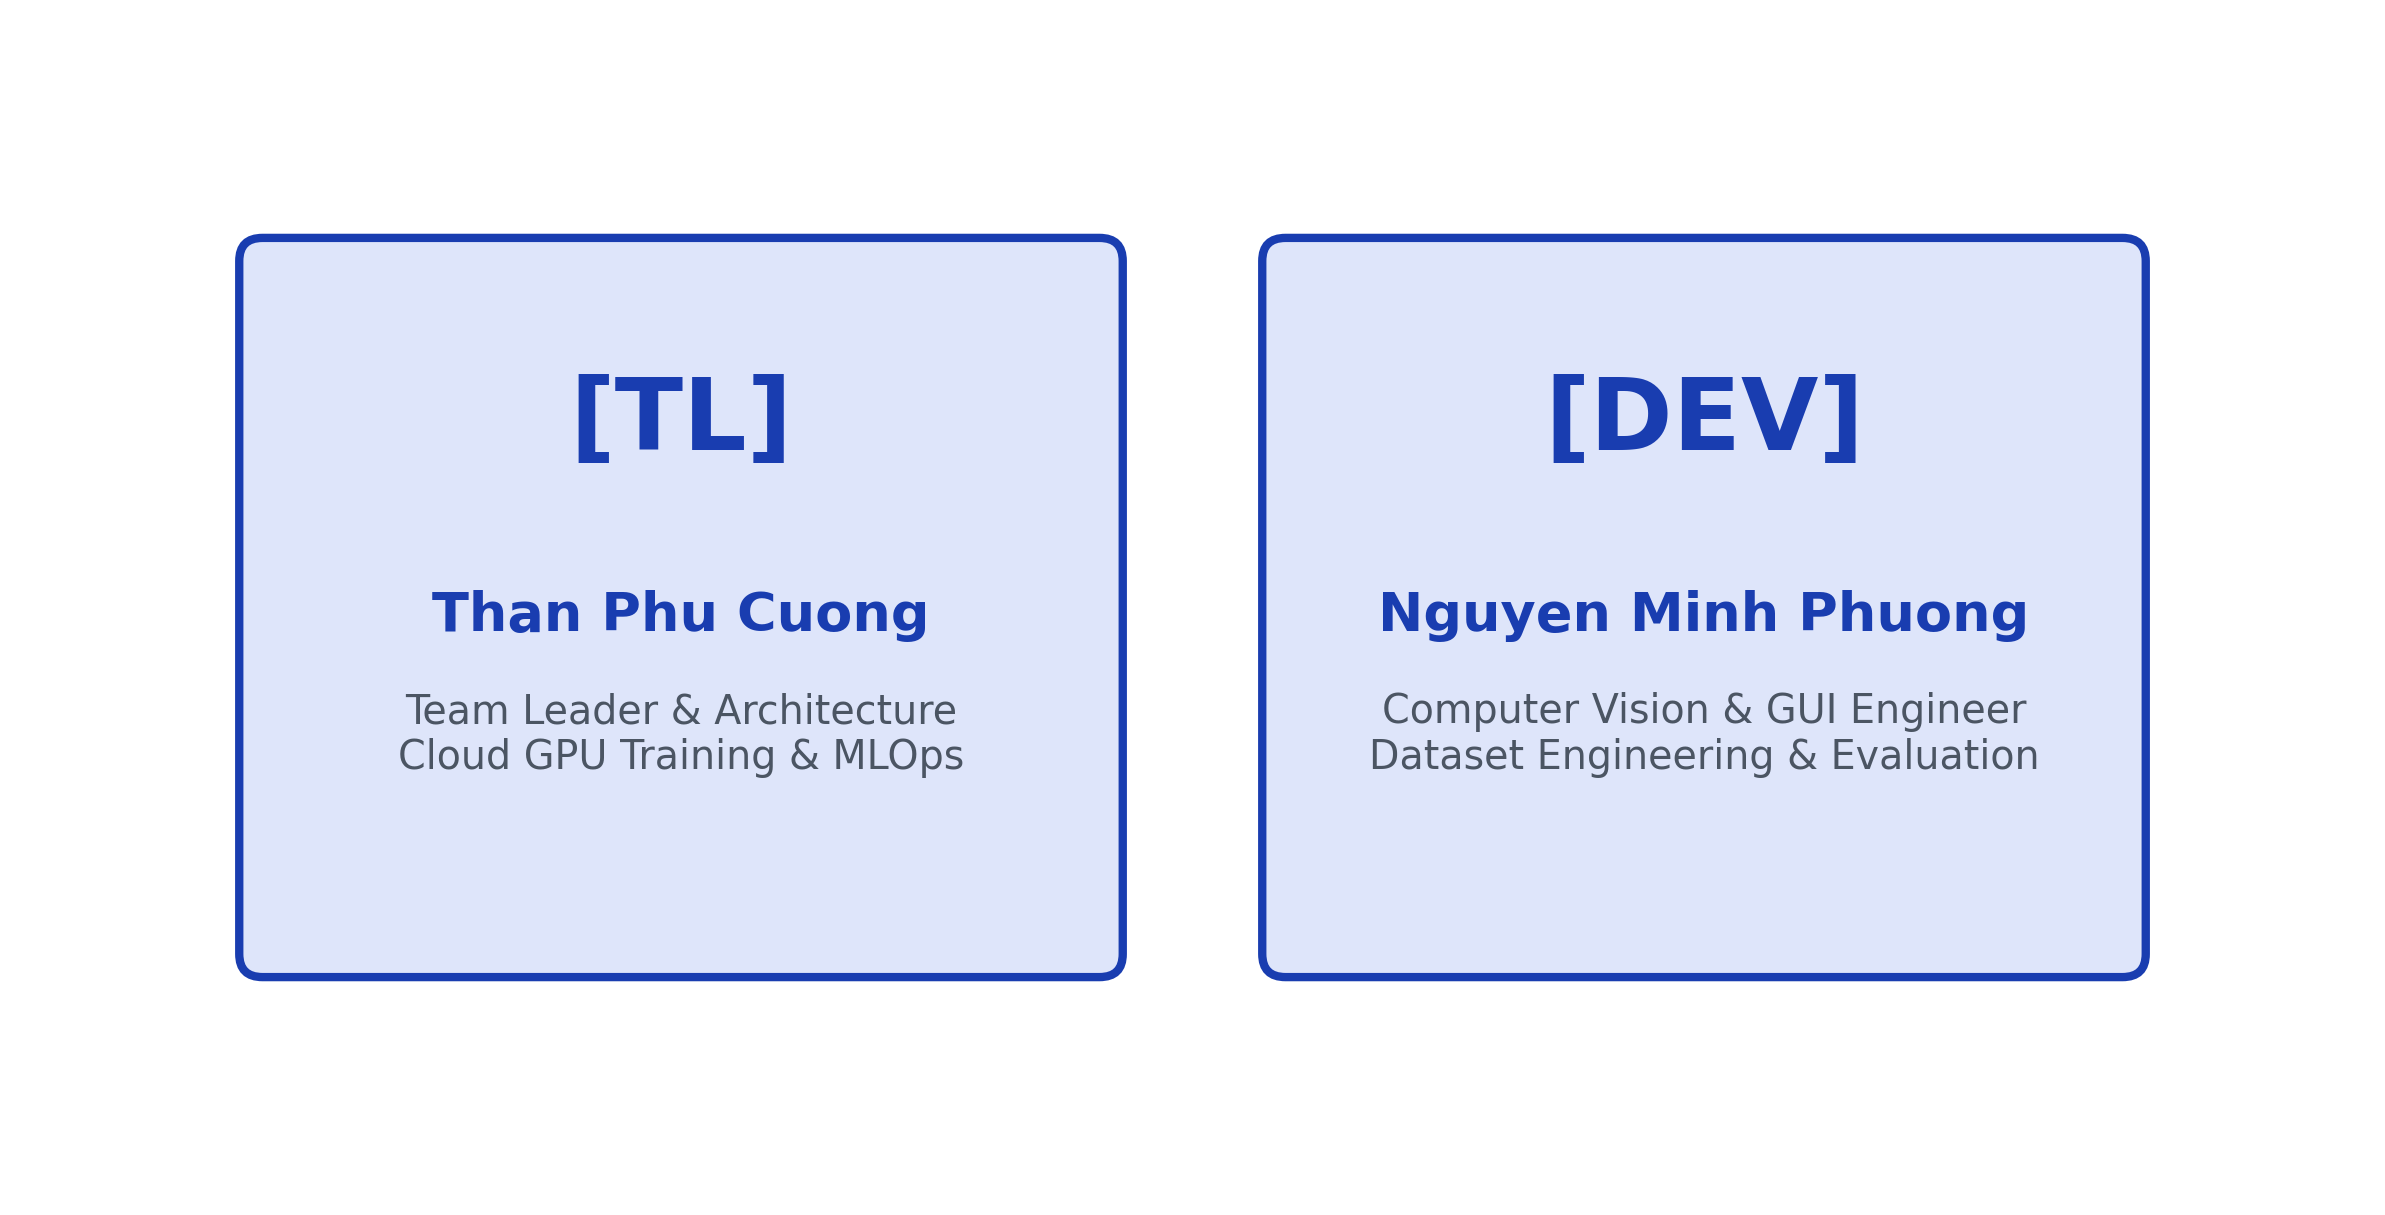
\includegraphics[width=0.88\textwidth]{figures/team_photo.png}
    \caption{Capstone Project Team Presentation and Member Contributions}
    \label{fig:team_photo}
\end{figure}

\vspace{0.3cm}

% ------------------------------------------------------------------------------
% TEAM MEMBERS REVIEW AND COMMENT TABLE
% Matches exact structure and palette of the source document (#DEE5FA fill, #BFBFBF borders)
% ------------------------------------------------------------------------------
\noindent
\begin{table}[htbp]
    \centering
    \caption{Individual Team Member Reviews and Comments}
    \label{tab:team_member_comments}
    \renewcommand{\arraystretch}{1.6}
    \arrayrulecolor{SamsungGray}
    \begin{tabularx}{\textwidth}{|>{\raggedright\arraybackslash\sffamily}p{3.8cm}|>{\raggedright\arraybackslash}X|}
        \hline
        \rowcolor{SamsungLightBlue}
        \multicolumn{1}{|c|}{\sffamily\bfseries\color{SamsungDarkGray}NAME} & 
        \multicolumn{1}{c|}{\sffamily\bfseries\color{SamsungDarkGray}REVIEW and COMMENT} \\
        \hline
        \textbf{\memberOne} & 
        Serving as Team Leader for the \textbf{Identify Anything} capstone project provided an exceptional opportunity to guide an end-to-end artificial intelligence engineering lifecycle. Designing the modular system architecture, orchestrating the cloud training workflow on Kaggle dual Tesla T4 GPUs, and developing the multi-threaded CustomTkinter desktop application gave me profound hands-on experience in modern AI software engineering. Bridging deep neural networks with real-time video streaming required careful concurrency management between OpenCV video buffering and PyTorch inference threads. Collaborating closely with my teammate enabled us to systematically reach our performance milestones and deliver a production-ready application operating at over 30 FPS. \\
        \hline
        \textbf{\memberTwo} & 
        My primary technical focus was centered on dataset engineering, mathematical loss analysis, and model optimization. Transforming complex hierarchical Supervisely JSON annotations into standardized YOLO bounding boxes required rigorous validation to eliminate geometric anomalies and scale disparities. Working with the Dollar Street dataset expanded my understanding of global AI equity, highlighting how diverse domestic living conditions affect visual object representations. Analyzing the mathematical mechanics of Complete IoU (CIoU) and Distribution Focal Loss (DFL) gave me deep theoretical insight into boundary regression under heavy visual occlusions. Achieving a peak validation mAP@0.50 of $96.4\%$ was immensely rewarding and validated our preprocessing and architectural choices. \\
        \hline
    \end{tabularx}
\end{table}
